\documentclass[journal,12pt,onecolumn]{IEEEtran}
\usepackage{cite}
\usepackage{caption}
\usepackage{graphicx}
\usepackage{amsmath,amssymb,amsfonts,amsthm}
\usepackage{algorithmic}
\usepackage{graphicx}
\usepackage{textcomp}
\usepackage{xcolor}
\usepackage{txfonts}
\usepackage{listings}
\usepackage{enumitem}
\usepackage{mathtools}
\usepackage{gensymb}
\usepackage{comment}
\usepackage[breaklinks=true]{hyperref}
\usepackage{tkz-euclide} 
\usepackage{listings}
\usepackage{gvv}
%\def\inputGnumericTable{}
\usepackage[latin1]{inputenc} 
\usetikzlibrary{arrows.meta, positioning}
\usepackage{xparse}
\usepackage{color}                                            
\usepackage{array}                                            
\usepackage{longtable}                                       
\usepackage{calc}                                             
\usepackage{multirow}
\usepackage{multicol}
\usepackage{hhline}                                           
\usepackage{ifthen}                                           
\usepackage{lscape}
\usepackage{tabularx}
\usepackage{array}
\usepackage{float}

\usepackage{float}
%\newcommand{\define}{\stackrel{\triangle}{=}}
\theoremstyle{remark}
\usepackage{circuitikz}
\captionsetup{justification=centering}
\usepackage{tikz}

\title{Matrices in Geometry 4.11.15}
\author{EE25BTECH11037 - Divyansh}
\begin{document}
\vspace{3cm}
\maketitle
{\let\newpage\relax\maketitle}
\textbf{Question: }
Find the equation of the plane which contains the line of intersection of the planes $\vec{r}\cdot\brak{ \hat{i}+2\hat{j} +3\hat{k}}-4=0$, $\vec{r}\cdot \brak{2\hat{i} + \hat{j} - \hat{k}} + 5 = 0$ and which is perpendicular to the plane $\vec{r}\cdot\brak{5\hat{i} +3\hat{j} - 6\hat{k}} +8 = 0.$
\vspace{2mm}

\textbf{Solution:}
 \vspace{1mm}
We need to find an equation of the plane that contains the line of intersection of the given two planes: 
\begin{align}
\vec{P_1}\  : \ \vec{n_1}^{\top}\vec{x}-4=0 \ \ , \vec{n_1}=\myvec{1 \\ 2 \\ 3 } \\
\vec{P_2} \ : \ \vec{n_2}^{\top}\vec{x}+5=0 \ \ , \vec{n_2}=\myvec{2 \\ 1 \\ -1 }
\end{align}
Another plane that passes through the intersection of these two planes is
\begin{align}
    \vec{P} \ : \ \vec{P_1} + \lambda\vec{P_2}=0 \\ 
    \vec{P} \ : \ \vec{n_1}^{\top}\vec{x}-4 + \lambda\brak{\vec{n_2}^{\top}\vec{x}+5}=0
\end{align}

This can be written as 
\begin{align}
    \vec{P} \ : \ \brak{\vec{n_1}^{\top}+ \lambda\vec{n_2}^{\top}}\vec{x} -4 + 5\lambda=0
\end{align}
The normal to this plane is 
\begin{align}
    \vec{n}=\vec{n_1} + \lambda\vec{n_2}
\end{align}

The plane $\vec{P}$ should also be perpendicular to the plane 
\begin{align}
    \vec{P_3} \ : \ \vec{n_3}^{\top} \vec{x}+8=0 \ , \ \vec{n_3}=\myvec{5 \\ 3 \\ -6} \\
    \therefore \vec{n_3}^{\top} \vec{n}=0 \implies \vec{n_3}^{\top}\brak{\vec{n_1} + \lambda\vec{n_2}}=0 \\
    \implies \vec{n_3}^{\top}\vec{n_1} + \lambda\vec{n_3}^{\top}\vec{n_2}=0\\
    \implies \myvec{5 & 3 & -6}\myvec{1 \\ 2 \\ 3 }  +  \lambda\myvec{5 & 3 & -6}\myvec{2 \\ 1 \\ -1 }=0 \\
    \implies -7 +19\lambda=0 \implies \lambda = \dfrac{7}{19}
\end{align}

Substituting this value of $\lambda$ in equation of $\vec{P}$, we get
\begin{align}
    \vec{P}\ :\ \brak{\myvec{1 & 2 & 3 } + \frac{7}{19}\myvec{2 & 1 & -1 }}\vec{x} -4 + \frac{35}{19}=0\\
    \vec{P} \ : \vec{n}^{\top}\vec{x}-41=0 \ , \ \vec{n}=\myvec{33 \\ 45 \\ 50}
\end{align}
\begin{figure}[H]
    \centering
    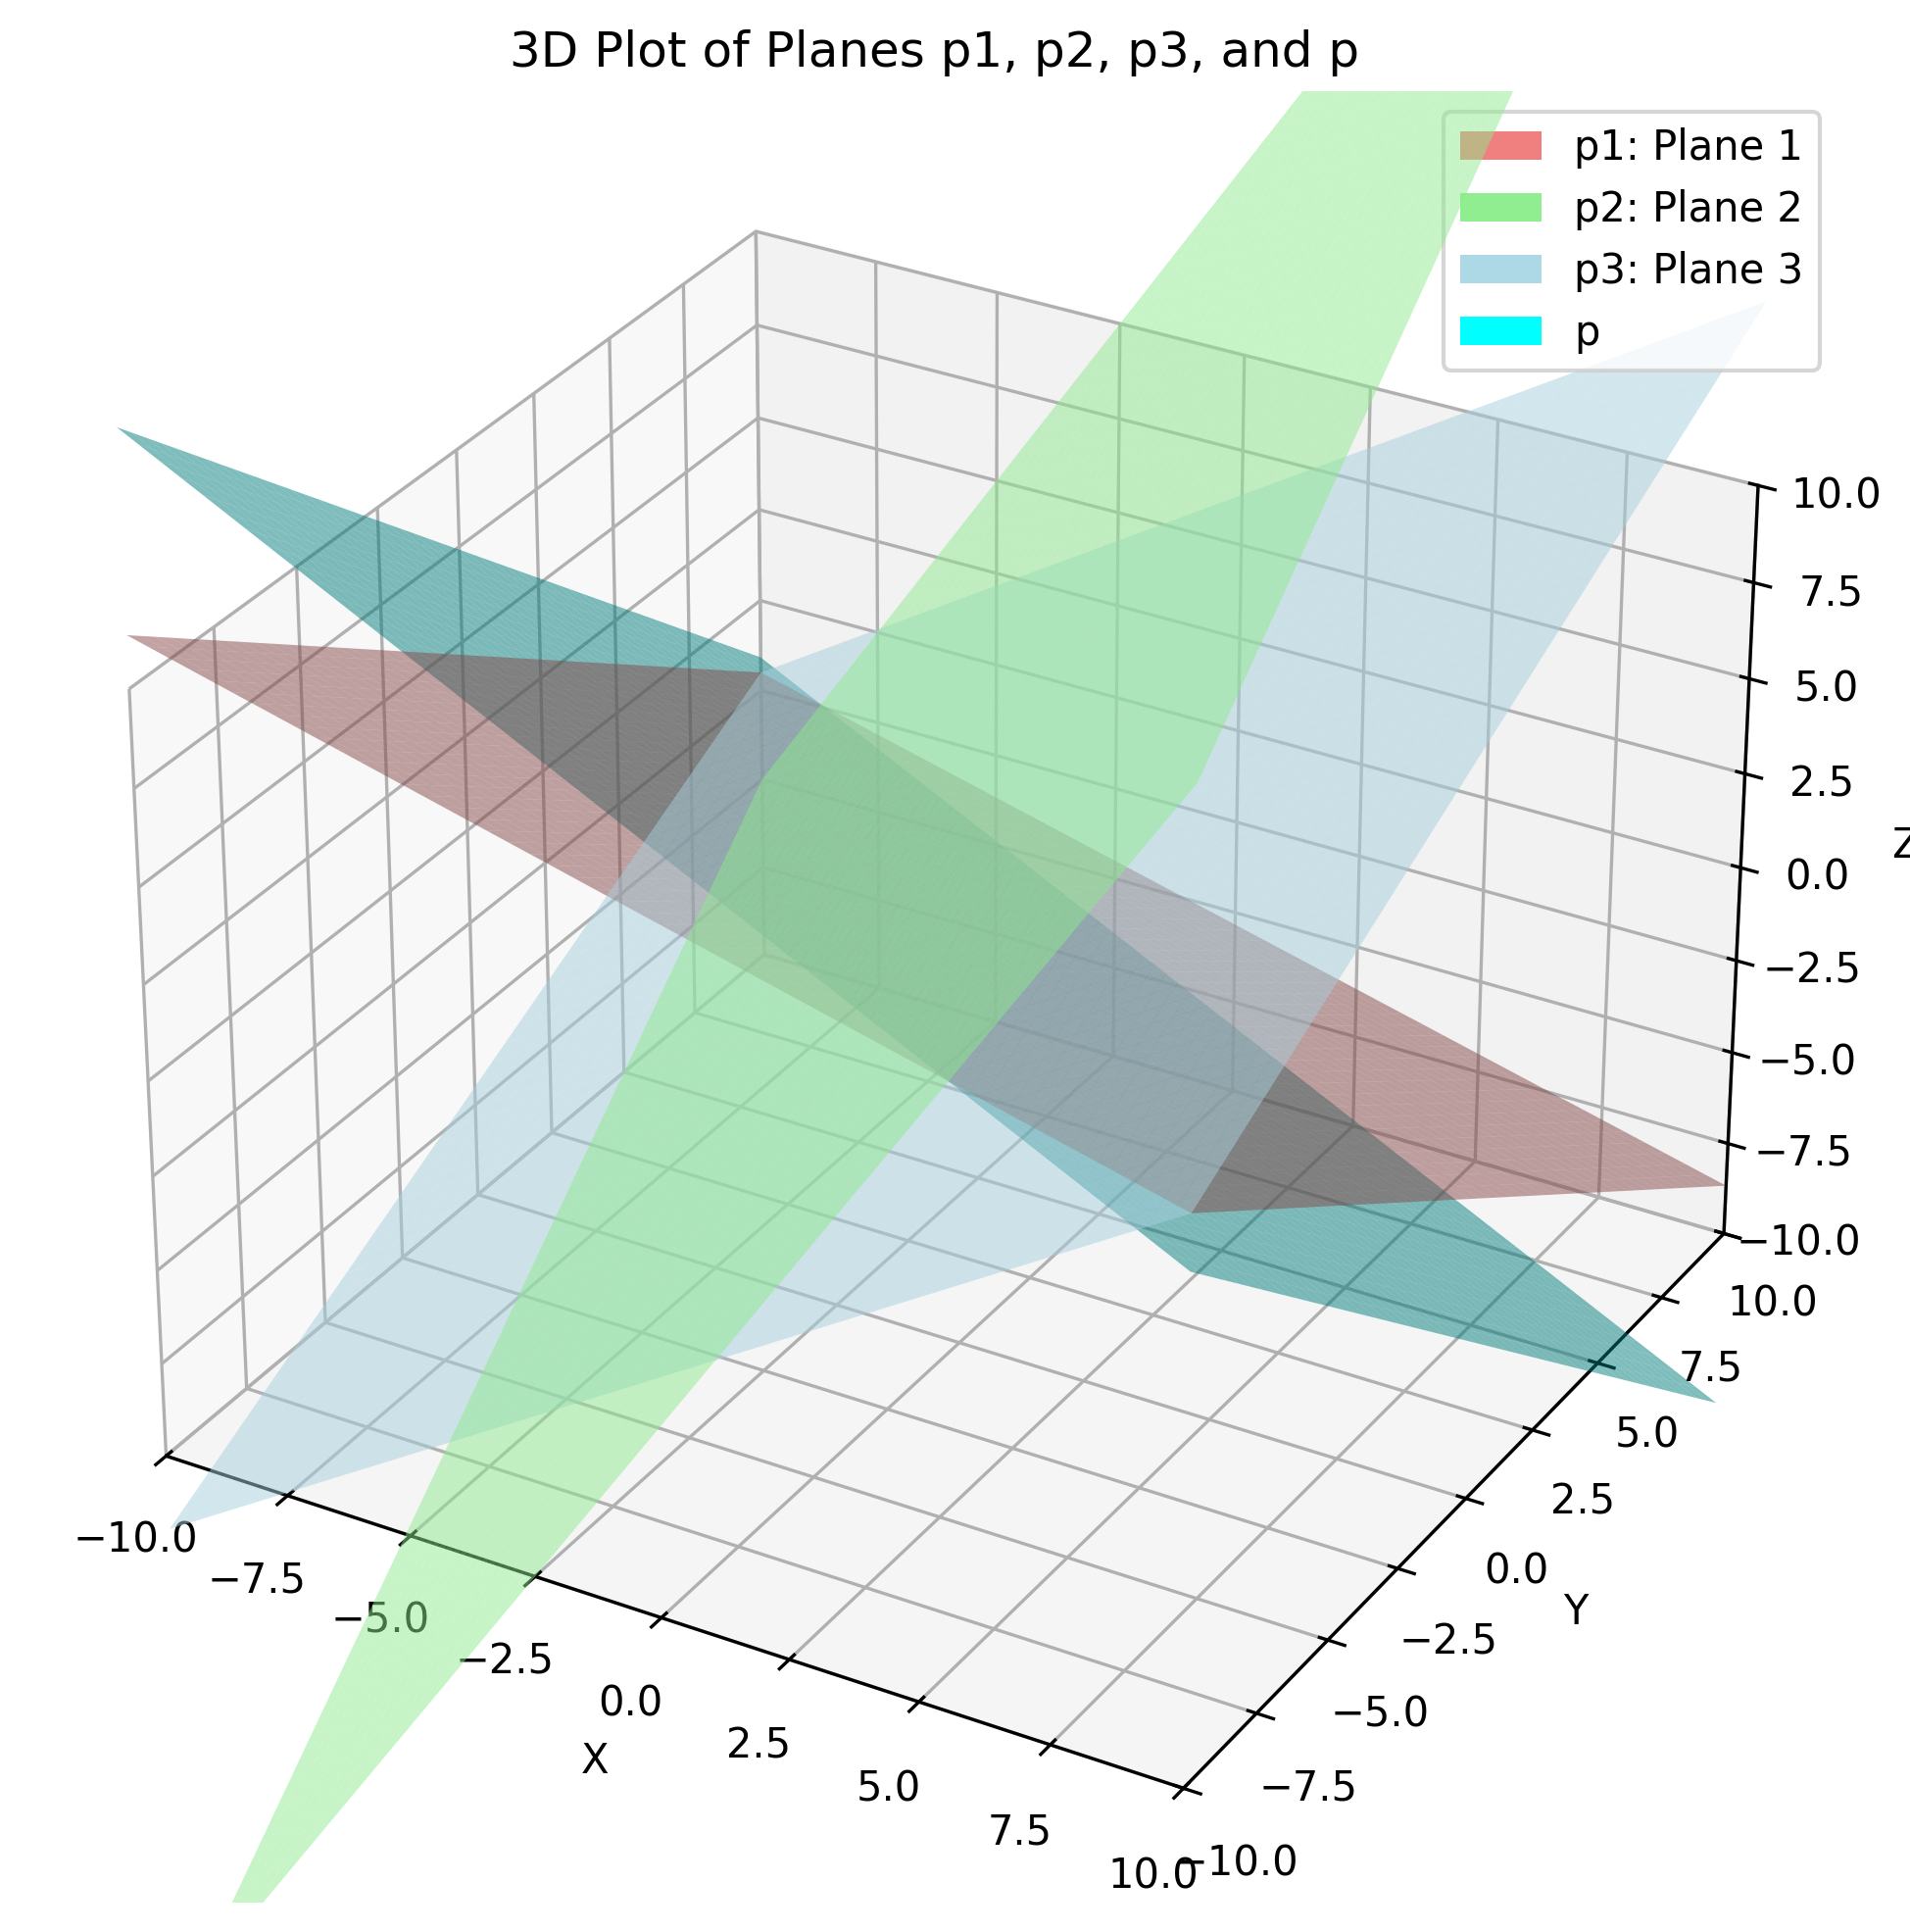
\includegraphics[width=1\columnwidth]{figs/1.png}
    \caption{Figure for 4.11.15}
    \label{fig:placeholder}
\end{figure}
\end{document}
